\section{Numerical Tests}\label{se:NumericalTests}

In this section we present numerical results obtained with the PD-ARS schemes in Section~\ref{se:TimeIntegration}.
The tests in Section \ref{se: Accuracy Tests} are designed to compare the accuracy of the schemes in streaming, absorption, and scattering-dominated regimes in one spatial dimension.
The test in Section \ref{se: Neutrino Stationary State Test} demonstrates the convex-invariance of PD-ARS schemes.
All the tests in this section were computed with third-order accurate spatial discretization (polynomials of degree $k=2$) and time step $\dt = 0.1 \times \dx $, using the DG scheme from~\cite{chu_etal_2018}.

\subsection{Accuracy Tests}
\label{se: Accuracy Tests}

To compare the accuracy of the IMEX schemes, we applied our PD-ARS schemes and the SSP2332 scheme from Pareschi \& Russo~\cite{pareschiRusso_2005} to problems with known smooth solutions in streaming, absorption (damping), and scattering-dominated (diffusing) regimes in one spatial dimension.
All the tests in this subsection were computed with the maximum entropy closure in the low-occupancy limit (i.e., the Minerbo closure).  
In the streaming test, the second- and third-order accurate explicit strong-stability-preserving Runge-Kutta methods from~\cite{gottlieb_etal_2001} (SSPRK2 and SSPRK3, respectively) are also included.  
To compare the numerical results to analytic solutions, the averaged absolute error or the averaged relative error are computed in the $L^{1}$-error norm.
We compute the absolute error for the streaming and diffusion tests and the relative error for the damping test.
They are averaged over the cell with an equal-weight quadrature for the cell integrals.
To examine the convergence, we let the number of elements ($N$) vary from 8 to 128.  

\subsubsection{Sine Wave Streaming}

The sine wave streaming test is designed to test accuracy in the free-steaming regime; i.e. $\sigma_{\Ab} = \sigma_{\Scatt} = 0$.
A periodic domain of unit length is used and the initial condition is $\cJ_{0} = \bcH_{0} = 0.5+0.49\times\sin\big(2\pi\,x\big)$.
We evolve the test until the sine wave has completed 10 crossings of the domain.
Figure~\ref{fig: SineWaveStreaming} plots the absolute error for the number density versus the number of elements $N$.
We see the errors obtained with SSPRK3 and PD-ARS3 are smallest and decrease as $N^{-3}$, as expected for a scheme combining third-order accurate time stepping with third-order accurate spatial discretization.
For all the other schemes, using second-order accurate explicit time stepping, the error decreases as $N^{-2}$.
Among the second-order schemes, SSP2332 has the smallest error.
In the streaming limit, the PD-ARS schemes reduce to SSPRK schemes --- PD-ARS2 to SSPRK2 and PD-ARS3 to SSPRK3, respectively.
Therefore, the absolute errors of PD-ARS schemes and SSPRK schemes are indistinguishable.  

\begin{figure}[h]
  \centering
    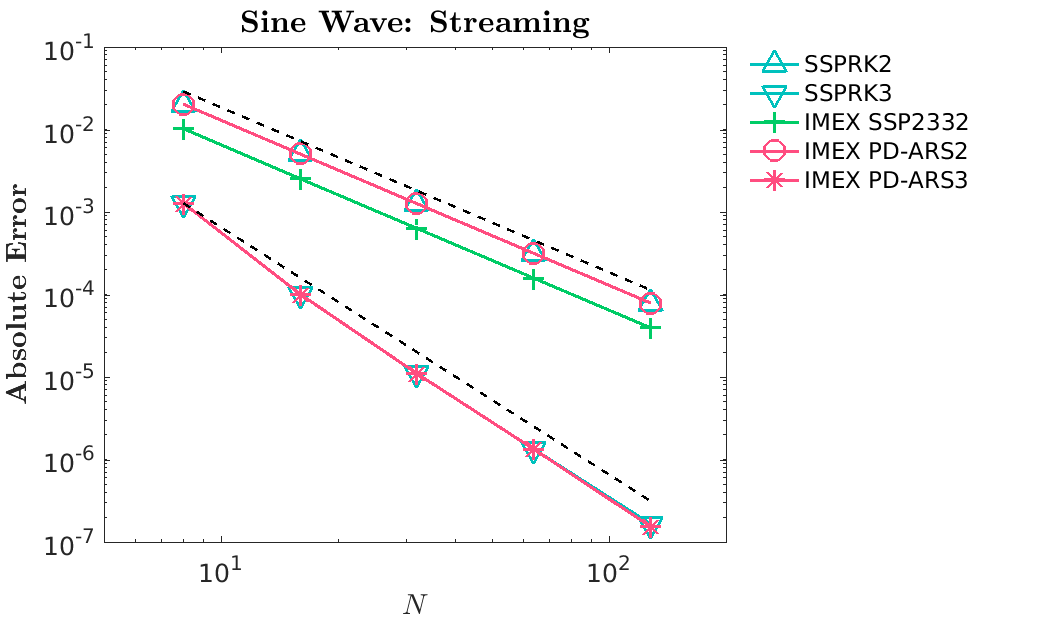
\includegraphics[width=0.8\textwidth]{figures/SineWaveStreaming}
   \caption{Absolute error versus number of elements, $N$, for the streaming sine wave test.  Results employing various time stepping schemes are compared: SSPRK2 (cyan triangles pointing up), SSPRK3 (cyan triangles pointing down), SSP2332 (green crosses), PD-ARS2 (light red circles) and PD-ARS3 (light red asterisks). Black dashed reference lines are proportional to $N^{-2}$ (top), and $N^{-3}$ (bottom), respectively.}
   \label{fig: SineWaveStreaming}
\end{figure}

\subsubsection{Sine Wave Damping}

The next test, adapted from~\cite{skinnerOstriker_2013}, is designed for absorption-dominated regimes, with $\sigma_{\Scatt} = 0$ and $f_0 = 0$, which results in exponential damping of the wave amplitude.
A periodic domain $D=\{x:x\in[0,1]\}$ and initial condition $\cJ_{0} = \bcH_{0} = 0.5+0.49\times\sin\big(2\pi\,x\big)$ are used.
The amplitude of the analytical solution decreases as $e^{-\sigma_{\Ab} t}$.
For $\sigma_{\Ab}$ = 0.1, 1 and 10 we evolve the test until the initial condition has been damped by a factor $e^{-10}$. 
Figure~\ref{fig:SineWaveDamping} shows convergence results of the test in the relative error.
Results for $\sigma_{\Ab}=0.1$, $1$, and $10$ are plotted with red, green, and blue lines, respectively.
SSP2332 is the most accurate among these schemes for $\sigma_{\Ab}= 1$ and 10. 
For $\sigma_{\Ab}=0.1$, PD-ARS2 is the most accurate scheme for $N=8$ and $N=16$. 
We have seen the same behavior for the scheme proposed by McClarren et al.~\cite{mcclarren_etal_2008} (PC2 in~\cite{chu_etal_2018}).
Since these are special cases for $N=8$ and $N=16$, we do not recommend PD-ARS2 instead of SSP2332 for the damping problem.
Only SSP2332, a second-order accurate scheme, displays a second-order convergence rate.  
The PD-ARS schemes are first-order accurate.

\begin{figure}[h]
  \centering
    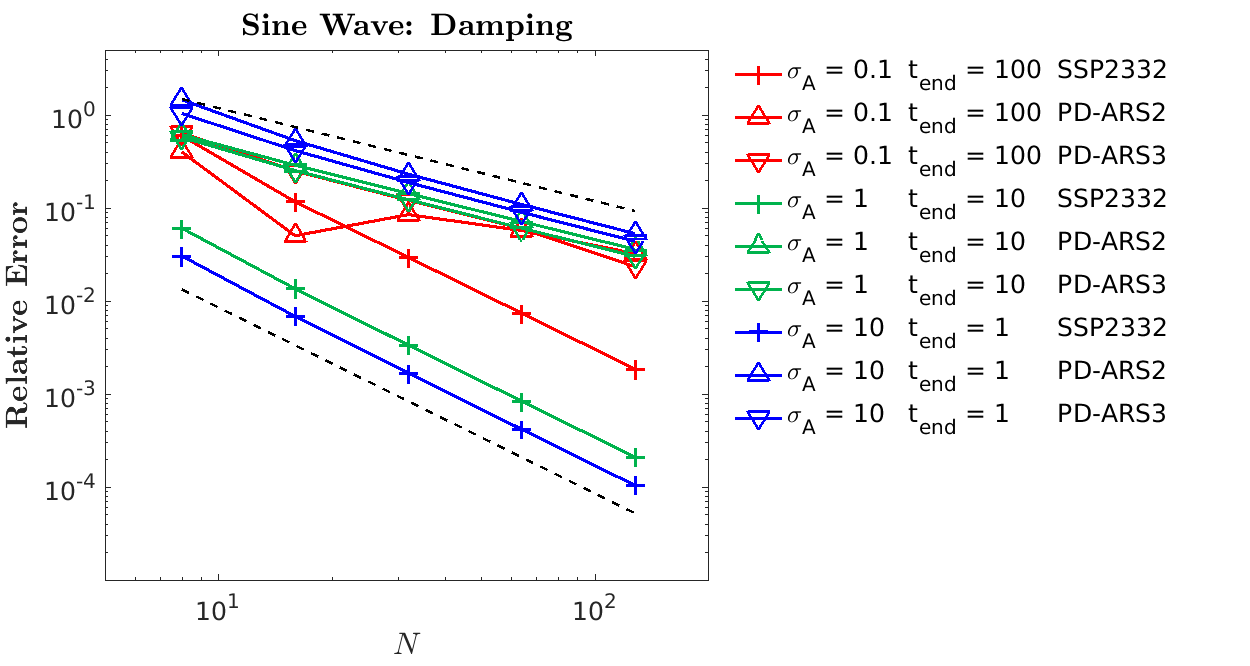
\includegraphics[width=0.9\textwidth]{figures/SineWaveDamping}
   \caption{Relative error versus number of elements, $N$, for the damping sine wave test. Results for different values of the absorption opacity $\sigma_{\Ab}$, employing various IMEX time stepping schemes, are compared.  Errors for $\sigma_{\Ab}=0.1$, $1$, and $10$ are plotted with red, green, and blue lines, respectively.  The IMEX schemes employed are SSP2332 ($+$), PD-ARS2 (triangles pointing up) and PD-ARS3 (triangles pointing down).  Black dashed reference lines are proportional to $N^{-1}$ (top) and $N^{-2}$ (bottom), respectively.}
  \label{fig:SineWaveDamping}
\end{figure}

\subsubsection{Sine Wave Diffusion}

The final test with known smooth solutions, adopted from~\cite{radice_etal_2013}, is the sine wave diffusion test; i.e. $\sigma_{\Ab} = 0$ and $f_0 = 0$.
A periodic domain $D=\{x:x\in[-3,3]\}$ with initial conditions $\cJ_{0} = 0.5+0.49\times\sin\big(\f{\pi\,x}{3}\big)$ and $\cH_{0} =-\f{1}{3\sigma_{\Scatt}}\pderiv{\cJ_{0}}{x}$ are used.  
The reference diffusion solution is given by $\cJ = \cJ_{0} \times \exp\big(-\f{\pi^2 t}{27\sigma_{\Scatt}}\big)$ and $\cH = (3\,\sigma_{\Scatt})^{-1}\pd{\cJ}{x}$.  
We evolve with $\sigma_{\Scatt}=10^{2}$, $10^{3}$, and $10^{4}$, and adjust the end time so that $t_{\mbox{\tiny end}}/\sigma_{\Scatt}=1$, 
at which time the amplitude of the sine wave has been reduced by a factor $e^{-\pi^{2}/27}\approx0.694$ for all values of $\sigma_{\Scatt}$. 
Figure~\ref{fig:SineWaveDiffusionJ} shows the absolute error, obtained using different values of $\sigma_{\Scatt}$, for various IMEX schemes at $t=t_{\mbox{\tiny end}}$, versus $N$. 
Results for $\sigma_{\Scatt}=10^{2}$, $10^{3}$, and $10^{4}$ are plotted with red, green, and blue lines, respectively.
SSP2332 and PD-ARS schemes display third-order accuracy for the number density, $\cJ$, and second-order accuracy for $\cH_{x}$, and their errors are difficult to distinguish.
For $\sigma=10^{2}$, the errors in the number density $\cJ$ do not drop below $10^{-6}$ because of differences between the two-moment model and the diffusion equation used to obtain the analytic solution.
For larger values of the scattering opacity, $\sigma=10^{3}$ or $10^{4}$, the two-moment model agrees better with the diffusion model, and we observe convergence over the entire range of $N$.
PD-ARS2 behaves as well as SSP2332 in the diffusion region but requires 33\% less implicit solves per time step.  

\begin{figure}[h]
  \centering
  \centerline{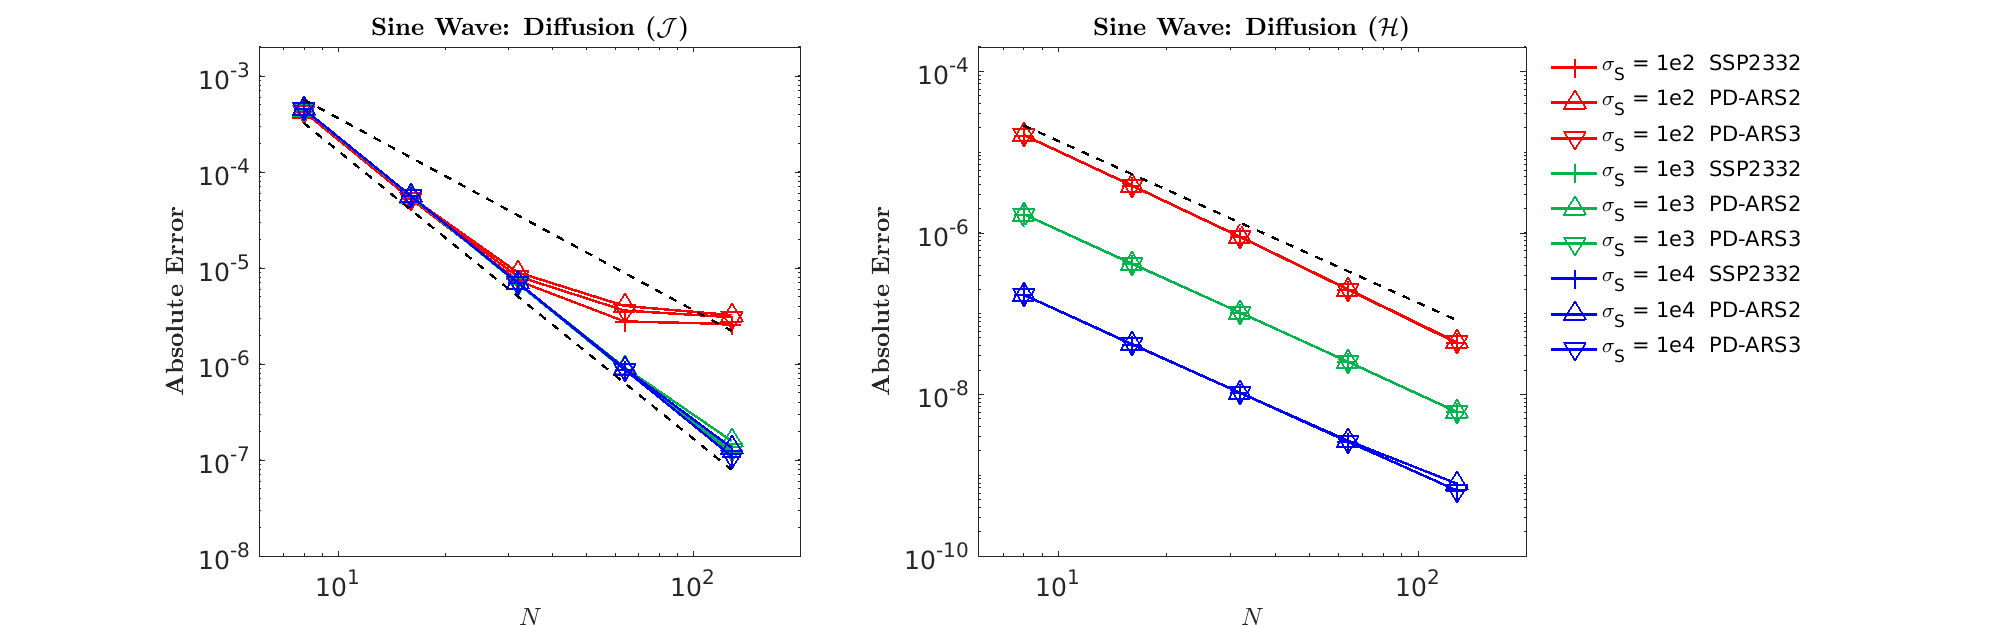
\includegraphics[width=1.2\textwidth]{figures/SineWaveDiffusion}}
   \caption{Absolute error for the number density $\cJ$ (left) and the number flux $\cH_{x}$ (right) versus number of elements for the sine wave diffusion test.  Results with different values of the scattering opacity, $\sigma_{\Scatt}$, employing different IMEX schemes, are compared.  Errors with $\sigma_{\Scatt}=10^{2}$, $10^{3}$, and $10^{4}$ are plotted with red, green, and blue lines, respectively.  The IMEX schemes employed are:  SSP2332 ($+$), PD-ARS2 (triangles pointing up), and PD-ARS3 (triangles pointing down). Black dashed lines in the left plot are reference lines proportional to $N^{-2}$ (top) and $N^{-3}$ (bottom), respectively. Black dashed line in the right plot is a reference line proportional to $N^{-2}$ .}
   \label{fig:SineWaveDiffusionJ}
\end{figure}

\subsection{Neutrino Stationary State Test} \label{se: Neutrino Stationary State Test}

In this section we consider a more ``realistic'' test: two-dimensional multigroup neutrino transport with emission, absorption, and isoenergetic scattering through a stationary background.  
This test is designed to test the realizability-preserving properties of the PD-ARS schemes.  
Figure~\ref{fig:NeutrinoStationaryTestEOS} left plots the initial thermal state: 
\begin{subequations}
\begin{align}
\text{Density: }~\rho & = 4 \times 10^{14} \times \dfrac{7.5}{( 7.5 + ( r / 5 )^4 )} ~\text{g $\cdot$ cm$^{-3}$}\\
\text{Temperature: }~T & = 1.5 \times 10^{11} \times \dfrac{1}{1 + ( r / 50 )^2 } ~\text{K}\\
\text{Electron Fraction: }~Y_e & = 0.25 \times \left(  1 + \dfrac{1}{1+ ( r / 50 )^{-12}}  \right) 
\end{align}
\label{eq:NuStatinaryStateEOS}
\end{subequations}
with radius $r$ in kilometer unit. 
Eq.~\eqref{eq:NuStatinaryStateEOS} is designed to simulate a CCSN progenitor.
Figure~\ref{fig:NeutrinoStationaryTestEOS} right plots the used opacities which are provided by interpolations of a pre-calculated opacity table based on~\cite{Bruenn_1985}.
This test is computed on Cartesian coordinate with a two-dimensional domain $D=\{\vect{x}\in\bbR^{2}:x^{1}\in[0,200], x^{2}\in[0,200]\}$ in kilometer unit, a grid of 128 elements in each direction, 10 energy groups covering $(0,300)$~MeV, a reflecting inner boundary and a homogeneous out-flowing outer boundary.
Because of the Cartesian coordinate, we ignored some geometric terms, which leads the initial condition to be non-axisymmetric.
We initialize the neutrino number density to $\cJ = 10^{-99}$, flux density to $\bcH=0$, and evolve until an approximate steady state is reached ($t=5$~ms).
No hydrodynamics is used for the stationary background.
For this test, we employed both CB and Minerbo closures.  
We attempted to run this test with our PD-ARS schemes, SSP2332 from~\cite{pareschiRusso_2005}, IMEXRKCB2 proposed by Cavaglieri \& Bewley~\cite{cavaglieriBewley2015}, and the IMEX PC2 scheme proposed by McClarren et al.~\cite{mcclarren_etal_2008}.
Only the PD-ARS schemes produce realizable moments and are able to evolve to a steady state with either CB or Minerbo closure.
SSP2332 and IMEX PC2 failed after a few time steps with either CB or Minerbo closure because of the development of unrealizable moments.
Even though IMEXRKCB2 with Minerbo closure can run and reach a steady state in this test, its results are different from that of PD-ARS schemes with CB closure, and there is no guarantee of stability.
%It's difficult to determine whether the results are in fact compromised by a particular correction step and, if so, in what way and to what degree.

Results obtained with the IMEX PD-ARS schemes are plotted in Figure~\ref{fig:NeutrinoStationaryTestEvolve} for various times: $t=0.01$~ms (top panels), 0.35~ms (middle panels), and 5.0~ms (bottom panels).  
In the left column we plot the solution in the $|\vect{\cH}|\cJ$-plane.  
In the middle column we show scatter plots of the number density $\cJ$ versus radius for select neutrino energies: 5~MeV (red lines), 16~MeV (magenta lines), and $93$~MeV (blue lines).  
In the right column we plot the flux factor $|\vect{\cH}|/\cJ$ versus radius for the same neutrino energies as in the middle column. 
In the left panels, each solution point in the domain is marked as a red dot in the $|\vect{\cH}|\cJ$-plane, and the realizable domain is shown as the light blue region.  
The figures show that all the states in the simulation with the PD-ARS schemes are realizable.
In the middle and right column, we can see how the neutrinos are generated near the core, stream out, and eventually reach an equilibrium distribution over the phase space.
The oscillation in the right column is caused by the oscillation in the numerical flux $|\vect{\cH}|$.
Parts of the causes can be the numerical error and the non-axisymmetric boundary condition.
We should also note that no flux limiter is used in this test.
The oscillation can be the spurious oscillations that occur due to discontinuities in the solution domain.
We leave these for our future study.

\begin{figure}[h]
  \centering
  \begin{tabular}{cc}
    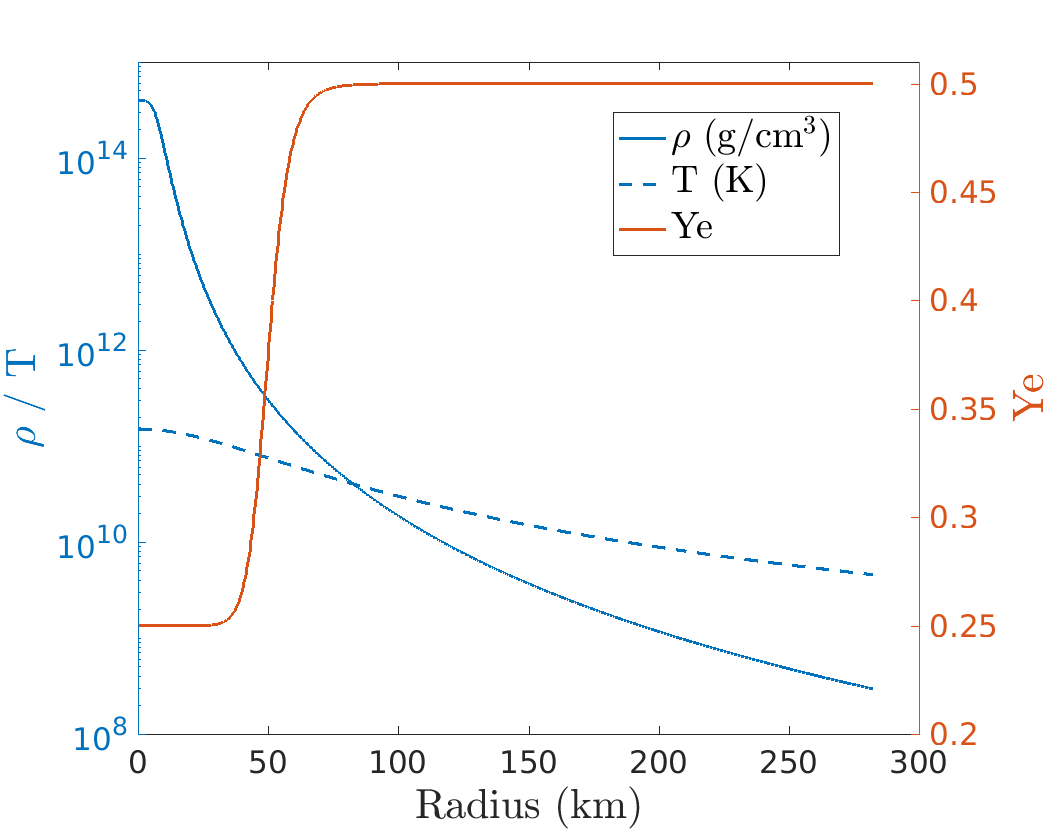
\includegraphics[width=0.45\textwidth]{figures/NStatinaryS_EOS}
    \hspace{30pt}
    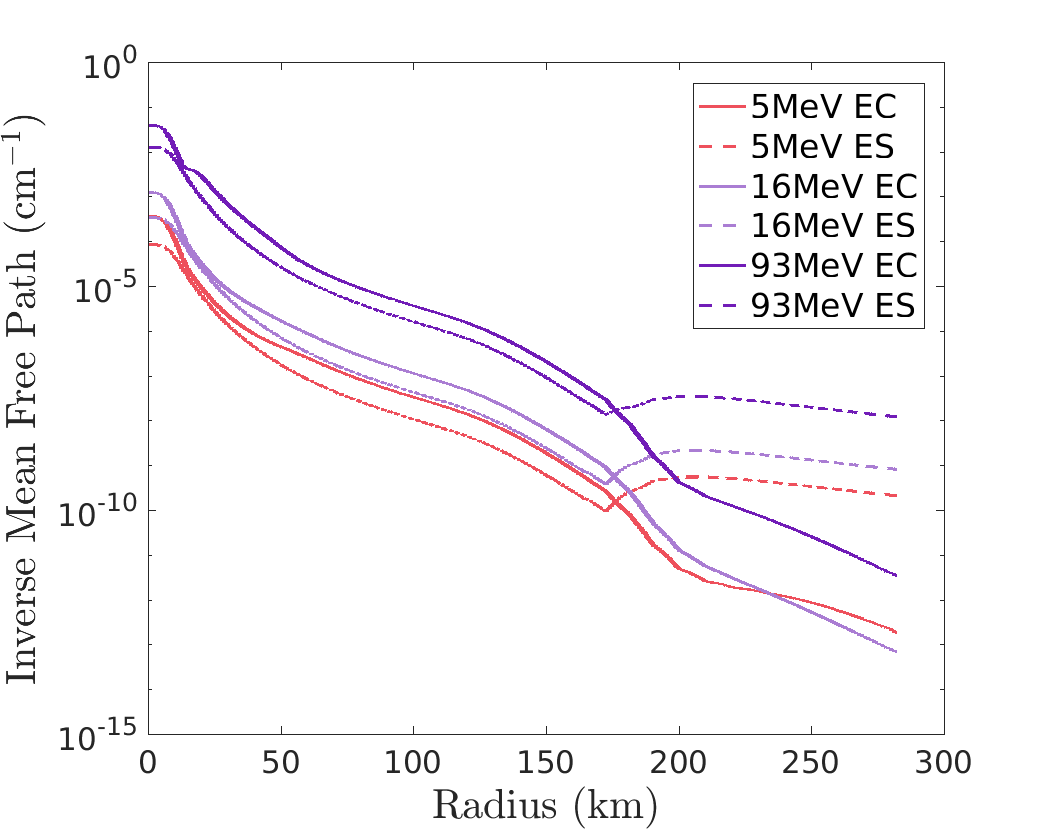
\includegraphics[width=0.45\textwidth]{figures/NSS_Opacities}
  \end{tabular}
   \caption{Left panel: thermal state of the background versus radius in the neutrino stationary state test; mass density (solid line), temperature (dashed line), and electron fraction (dotted line).  Right panel: corresponding opacities for select neutrino energies; absorptivity ($\sigma_{\Ab}$) and scattering opacity ($ \sigma_{\Scatt}$).}
   \label{fig:NeutrinoStationaryTestEOS}
\end{figure}

\begin{figure}[h]
  \centering
    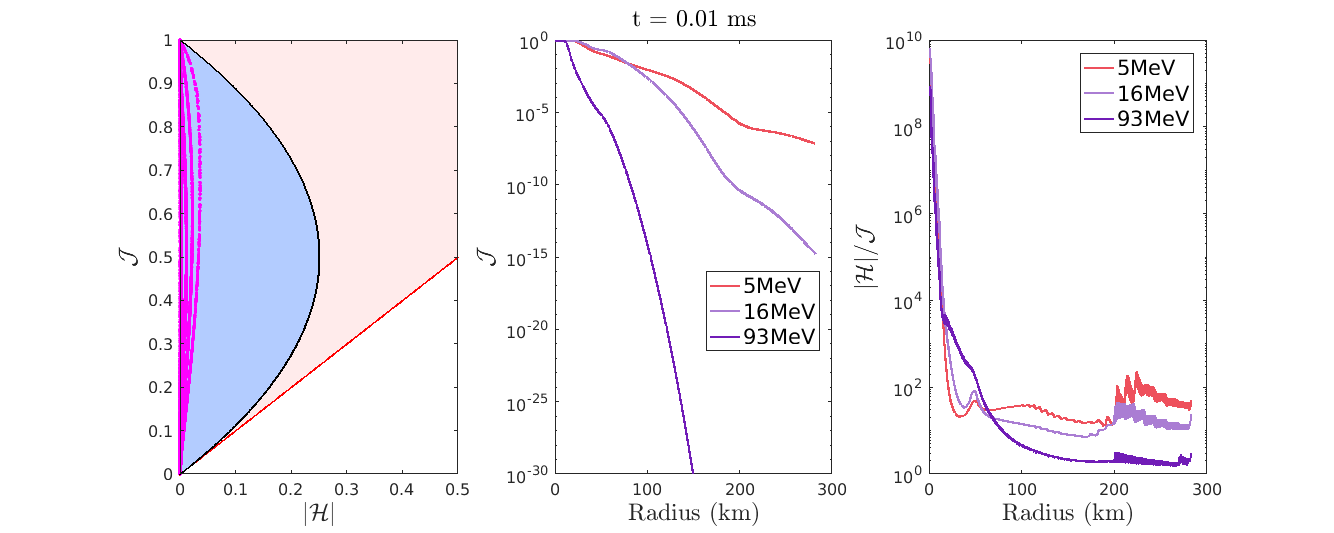
\includegraphics[width=.9\textwidth]{figures/NSS_1_1}\\
    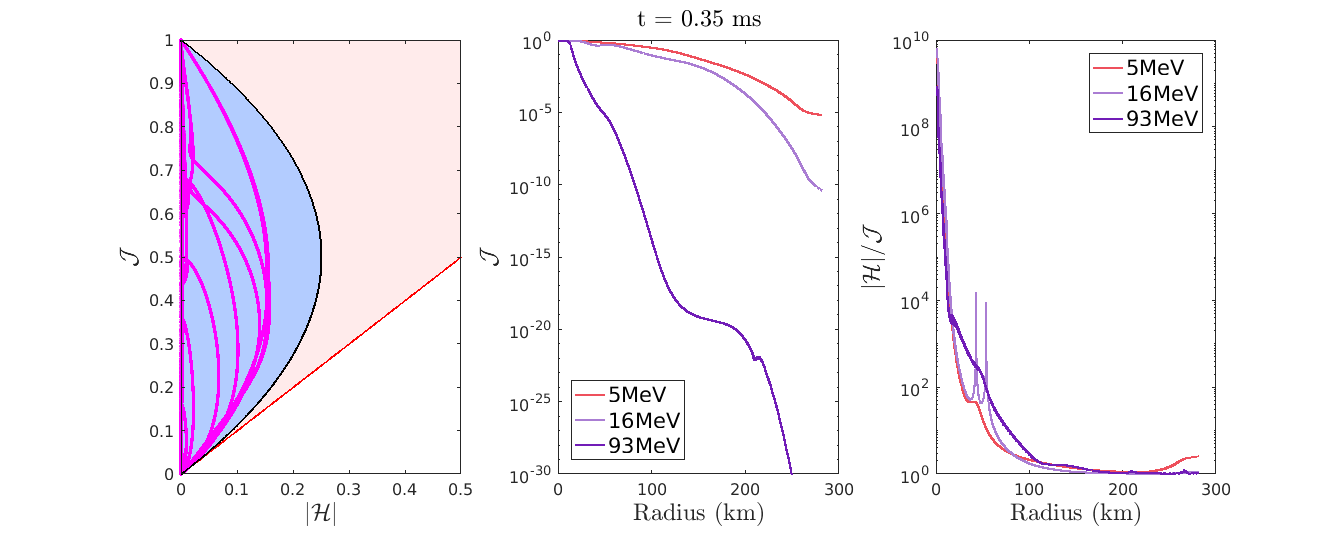
\includegraphics[width=.9\textwidth]{figures/NSS_3_1} \\
    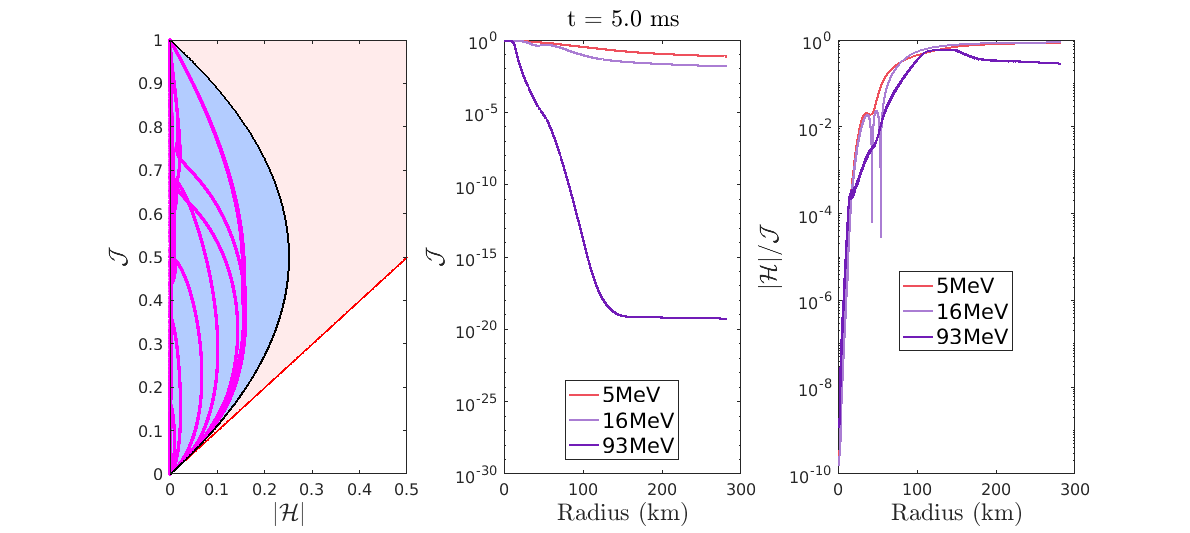
\includegraphics[width=.9\textwidth]{figures/NSS_5_1} \\
    \caption{Results from the neutrino stationary state test: moments relative to the realizable domain (left column, the light blue domain is for $f \in [0,1]$, with the black-solid-line as its boundary, while the light red domain is for $f\geq 0$, with the thin-red-solid-line as its boundary), the number density $\cJ$ versus radius (middle column), and the flux factor $|\bcH|/\cJ$ versus radius (right column), at $t = 0.01$~ms, 0.35~ms, and 5.0~ms.  For the plots in the left column, each $\bcM=(\cJ,\bcH)^{T}$ state is marked by a red dot, which are all inside the light blue region (the realizable domain for fermions).  The results of PD-ARS2 and PD-ARS3 are indistinguishable in these plots.}
    \label{fig:NeutrinoStationaryTestEvolve}
\end{figure}